\documentclass[tikz,border=10pt]{standalone}
\usetikzlibrary{intersections,calc}

\begin{document}
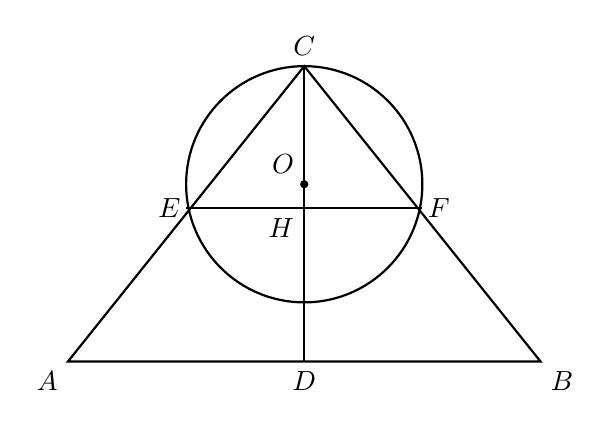
\begin{tikzpicture}[thick, scale=1.5]
    % 1. 定义核心点坐标
    \coordinate (A) at (0,0);
    \coordinate (B) at (4,0);
    \coordinate (C) at (2,2.5);
    \coordinate (O) at (2,1.5); % 圆心位置
    
    % 2. 绘制大三角形 ABC
    \draw (A) -- (B) -- (C) -- cycle;
    
    % 3. 绘制圆 O
    \def\radius{1}
    \draw (O) circle (\radius);
    \fill (O) circle (1pt) node[above left] {$O$};
    
    % 4. 计算特殊点
    % D是圆与AB附近的垂足点
    \coordinate (D) at (2,0);
    \draw (C) -- (D);
    
    % 定义直线 EF (穿过圆心 O)
    % 这里使用角度设定直线斜率，模拟图像中的横贯线
    \draw[name path=EF] (1, 1.3) -- (3, 1.3);
    
    % 求交点 E, F, H
    \path[name path=AC] (A) -- (C);
    \path[name path=BC] (B) -- (C);
    \path[name path=CD] (C) -- (D);
    
    \path [name intersections={of=EF and AC, by=E}];
    \path [name intersections={of=EF and BC, by=F}];
    \path [name intersections={of=EF and CD, by=H}];
    
    % 5. 绘制剩余线条
    \draw (E) -- (F);
    
    % 6. 标注节点名称
    \node[below left] at (A) {$A$};
    \node[below right] at (B) {$B$};
    \node[above] at (C) {$C$};
    \node[below] at (D) {$D$};
    \node[left] at (E) {$E$};
    \node[right] at (F) {$F$};
    \node[below left] at (H) {$H$};
    
\end{tikzpicture}
\end{document}